\documentclass[11pt]{article}
\usepackage[margin=1in]{geometry}
\usepackage{amsmath}
\usepackage{amssymb}
\usepackage{graphicx}
\usepackage{tikz}
\usetikzlibrary{positioning}

\title{DSC 257R: Unsupervised learning\\Homework 7\\Markov random fields and energy-based models}
\author{}
\date{}

\begin{document}

\maketitle

\begin{enumerate}

\item Probability distribution $P$ over binary variables $x_1, \ldots, x_6 \in \{0, 1\}$ has the following form:
\[
P(x_1, \ldots, x_6) = \frac{1}{Z} \psi(x_1, x_2)\psi(x_2, x_3)\psi(x_3, x_4)\psi(x_4, x_5)\psi(x_5, x_6)\psi(x_6, x_1)
\]
where for $a, b \in \{0, 1\}$,
\[
\psi(a, b) = \begin{cases}
1 & \text{if } a = b\\
0.5 & \text{otherwise}
\end{cases}
\]

\begin{enumerate}
\item Draw the minimal undirected graph $G$ over which $P$ factors. (This is the undirected graph with the fewest possible edges that contains cliques corresponding to each of the terms in $P$.)

\item For what configuration(s) $x \in \{0, 1\}^6$ is $P(x)$ maximized?

\item For what configuration(s) $x \in \{0, 1\}^6$ is $P(x)$ minimized?
\end{enumerate}

\item In a tournament, each player plays three games. Define three random variables:
\begin{itemize}
\item Random variable $A$ is 1 if Tom wins his first game, and is 0 otherwise.
\item Random variable $B$ is 1 if Tom wins his first two games, and is 0 otherwise.
\item Random variable $C$ is 1 if Tom wins all three of his games, and is 0 otherwise.
\end{itemize}

\begin{enumerate}
\item Is $C$ independent of $A$ (i.e., is it true that for any values $a, c$ that $A, C$ might take on, we have $\Pr(A = a, C = c) = \Pr(A = a)\Pr(C = c)$)? Give a brief (one-sentence) reason for your answer.

Hint: The answer is no; show this by exhibiting specific choices of $a, c$ for which $\Pr(A = a, C = c) \neq \Pr(A = a)\Pr(C = c)$.

\item Is $C$ conditionally independent of $A$ given $B$ (i.e., is it true that $\Pr(C = c|A = a, B = b) = \Pr(C = c|B = b)$)? Give a brief reason.

\item Draw an undirected graphical model for $(A, B, C)$.
\end{enumerate}

\newpage

\item Four random variables $W, X, Y, Z$ factor over the graph shown below.

\begin{center}
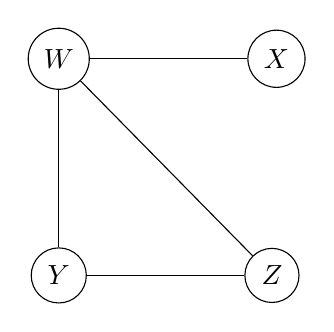
\begin{tikzpicture}[node distance=2cm]
\node[circle,draw] (W) {$W$};
\node[circle,draw,right=of W] (X) {$X$};
\node[circle,draw,below=of W] (Y) {$Y$};
\node[circle,draw,right=of Y] (Z) {$Z$};
\draw (W) -- (X);
\draw (Y) -- (W);
\draw (Y) -- (Z);
\draw (W) -- (Z);
\end{tikzpicture}
\end{center}

\begin{enumerate}
\item What is the functional form of the joint distribution $P(W, X, Y, Z)$?

\item Write down a conditional independence property of this distribution.
\end{enumerate}

\item The joint distribution $P$ over $(x_1, x_2, x_3)$ is given by the following table.

\begin{center}
\begin{tabular}{c|c|c|c}
$x_1$ & $x_2$ & $x_3$ & Pr \\\hline
0 & 0 & 0 & 1/3 \\
0 & 0 & 1 & 1/3 \\
1 & 0 & 0 & 1/6 \\
1 & 1 & 1 & 1/6
\end{tabular}
\end{center}

\begin{enumerate}
\item One of these variables is a deterministic function of the other two. Identify this relationship.

\item Draw the minimal Bayes net $G$ over which this distribution factors. Hint: Start from (a), which shows that one variable is fully determined by the other two; are the latter two variables independent or not?

\item Now show how $P$ factors over $G$ by explicitly giving the three (conditional) probability tables, one per $x_i$.

\item Draw the minimal undirected graph $G'$ over which distribution $P$ factors.
\end{enumerate}

\item A Bayesian approach to image denoising. Download the file \texttt{gibbs.zip} from the course website. This contains a Jupyter notebook and two images (\texttt{noisy\_bear.png} and \texttt{original\_bear.png}). The former is a corrupted version of the latter (which is provided only for reference).

Let $X$ be the corrupted image and $Y$ the uncorrupted version that we wish to recover. Both are of the form $\{-1, +1\}^{M \times N}$. In the notebook, a Markov random field joint distribution for $(X, Y)$ is given. You will use this to design a Gibbs sampler for $Y|X$.

\begin{enumerate}
\item Let $p$ denote a specific pixel in the image. Then $Y_p$ is the (reconstructed) value at that pixel, and $Y_{\backslash p}$ is the value at all remaining pixels. Give a precise expression for $\Pr(Y_p = +1|Y_{\backslash p}, X)$.

\item Implement a Gibbs sampler at the appropriate place in the notebook. Initialize $Y$ by setting each pixel to $\{-1, +1\}$ uniformly at random. Then apply the sampler and show the image $Y$ at various stages while the Markov chain is mixing: show any five of the images obtained along the way.

\item To reconstruct the image, just set the value of each pixel $p$ to $\mathbb{E}[Y_p|X]$. Show this image.
\end{enumerate}

\item Rejection sampling. Suppose we want to sample from a one-dimensional density $f(x)$ for which we do not have a readymade sampler. One way to do this is via rejection sampling. Here's the idea:
\begin{itemize}
\item We choose another distribution $g(x)$ from which we know how to sample (e.g. uniform or Gaussian distribution). We will call this the proposal distribution. It is important that $g(x)$ be nonzero whenever $f(x)$ is nonzero.
\item Let $M$ be an upper bound on $f(x)/g(x)$; that is, $f(x)/g(x) \leq M$ for all $x$.
\item To generate a sample from $f$, we repeat the following procedure until it accepts:
\begin{itemize}
\item Generate a sample $x$ from $g$
\item With probability $f(x)/(Mg(x))$, accept the sample. Otherwise, reject it.
\end{itemize}
\end{itemize}

Let's see how this works in practice. Let's say we want to sample a number in the range $[0, \pi]$ from
\[
f(x) = \frac{1}{2} \sin x
\]
(think of $x$ as being in radians).

\begin{enumerate}
\item Plot the density of $f$.

\item Give a suitable proposal distribution $g(x)$. What is a suitable upper bound $M$ on $f(x)/g(x)$?

\item Use rejection sampling to generate 10000 samples from $f$. How many times did you need to sample from $g$?

\item Plot the histogram of the samples you generated, using 50 bins. It should bear a resemblance to the density in (a).
\end{enumerate}

\end{enumerate}

\end{document}
